\documentclass[a4paper,12pt]{book}
\bibliographystyle{junsrt}
\usepackage{ascmac}
\usepackage{empheq}
\usepackage{amsmath,amssymb}
\usepackage{bm}
\usepackage[dvipdfmx]{graphicx,color,hyperref}
\usepackage[top=30truemm,bottom=30truemm,left=30truemm,right=30truemm]{geometry}
\usepackage{braket}
\usepackage{here}
\usepackage{comment}
\usepackage{jtygm} % Warning
\usepackage[hang,small,bf]{caption}
\usepackage[subrefformat=parens]{subcaption}
\captionsetup{compatibility=false}
\title{Seismic Noise Under the Ground}
\author{Koseki Miyo}

% ハイパーリンクを付ける設定
\usepackage{pxjahyper}
\hypersetup{
  colorlinks=true,
  linkcolor=blue,
  %bookmarks=true, 
  bookmarksnumbered=true,
  pdfborder={0 0 0},
  bookmarkstype=toc
}


\begin{document}
\setcounter{tocdepth}{2}
\maketitle

\tableofcontents

\chapter{Seismic Noise Under the Ground}
\section{Introduction}
\subsection{Site on the Ground Surface}
\subsection{Site under the Ground}
\subsection{KAGRA Site}
\section{Theory of Seismic Waves}
\subsection{Seismic Waves}
\subsection{Depth Dependence}
\subsection{...}
\section{Seismic Noise}
\subsection{Problematic Seismic Noise}
\subsection{The Microseisms}

\subsection{The Earth Quakes}
I have to explain how earth quake shake the KAGRA site and how serious for interferometer.
\begin{itemize}
\item 
\item Mechanism and frequency of earthquake?
\end{itemize}

\subsection{The Earth Tide}

\begin{itemize}
  \item To explain accuracy of GIF in low frewuency comparign with seismometers, This subsection describe about the measurement of the Earth Tide using GIF, which is consistent with the GOTIC model.
\end{itemize}

\subsection{...}
\section{Differential Motion Reduction}
\subsection{Introduction}
The seismic noise shakes both the common and the differential motion of the arm baseline. The common motion moves the center of mass of that, and the differential motion changes the arm length. Amplitudes of these are the same each other, when the two points in the arm moves with no correlation. However, if there are some coherencies, the differential motion is less than the common motion. It is important property of the ground for controling the arm length.

The coherence depends on both the arm length and the wave length of seismic waves, which is discussed in this section. For example, if the arm length is much smaller than the wave length, the two points move together. It means that the common motion is greater than the differential motion. Additionally, the wave length differs depending on the phase velocity of the seismic waves on the ground. Especially in KAGRA, the velocity is much higher than other sites because of the gneiss in the mine.

A ratio of the amplitudes of the differential motion over common motion is defined as Common and Differential Motion Ratio (CDMR). It is usefull to know how the groung reduct the differential motion or increase the common motion.

In fact, we need to consider about the common motion; because the arm length fluctuation is caused by not only the disturbance from the differential motion but also the coupling from the common motion. This coupling ratio is known as the Common Mode Rejection Ratio (CMRR). This is defined as the ratio of the powers of the differential-mode response over the common-mode response in a system.

In this section, CDMR is discussed in detail, while CMRR is not disscused.

\subsection{Differential Motion Reduction}
\subsubsection{Differential Motion and Common Motion}
\begin{figure}[H]
  \begin{center}
    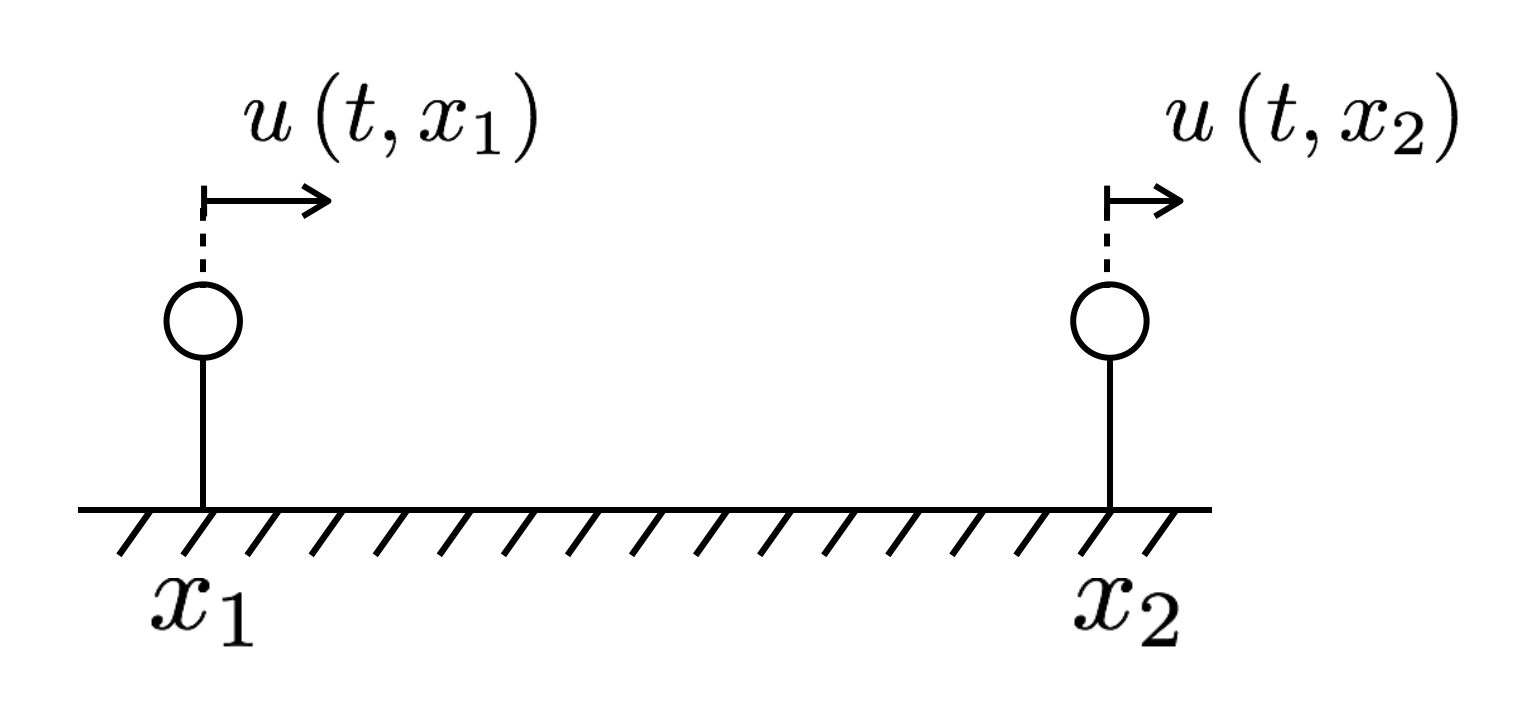
\includegraphics[width=8.0cm]{./img_cdmr_arm.png}
  \end{center}
  \caption{Displacements of the two points,$x_1,\,x_2$. Displacements of each point are represented as $u(x_1,t),\, u(x_2,t)$, in the case displacement field is given with $u(x,t)$, where $x$ is point of the point and $t$ is a time.
  }\label{img:img_diffcomm}  
\end{figure}
Motions of the two points can be represented as the differential motion and the common motion. Displacement of both differential motion and common motion of the two points shown in Figure\ref{img:img_diffcomm} is defined as
\begin{eqnarray}\label{eq:eq22}
  u_{\mathrm{diff}} \equiv \frac{u_{1}-u_{2}}{\sqrt{2}}, \,
  u_{\mathrm{comm}}  \equiv \frac{u_{1}+u_{2}}{\sqrt{2}}
\end{eqnarray}
where $u_{1}(x,t)$ and $u_2(x,t)$ are the displacement in each points.



\subsubsection{Common and Differential Motion Ratio (CDMR)}
Common and Differential Motion Ratio (CDMR) is defined as the powers of common motion over the differential motion as bellow,
\begin{equation}
  \mathrm{CDMR} \equiv \sqrt{\frac{\mathrm{Common\,Motion}}{\mathrm{Differential\,Motion}}} = \sqrt{\frac{P_{\mathrm{comm}}(\omega)}{P_{\mathrm{diff}}(\omega)}} \label{eq:eq23}
\end{equation}
where $P_{\mathrm{comm}},P_{\mathrm{diff}}$ is the power spectrum densities (PSDs) of them. These are estimated by the autocorrelation function of these with the Wiener-Khinchin theorem.

Autocorrelation function $C_{\mathrm{diff}}$ is given by
\begin{eqnarray}
  C_{\mathrm{diff}}(\tau) &=& \frac{1}{2}
  \biggl\langle
  \biggl[ x_{1}(t)-x_{2}(t) \biggr] \biggl[ x_{1}(t+\tau)-x_{2}(t+\tau) \biggr]
  \biggr\rangle \\
  &=& \frac{1}{2}\biggl[ C_{11}(\tau) - C_{12}(\tau) - C_{21}(\tau) + C_{22}(\tau) \biggr], 
\end{eqnarray}
,where $C_{ij}$ are the autocorrelation functions of each point and defined as $ C_{ij} \equiv \langle x_{i}(t)x_{j}(t+\tau)\rangle,\, (i=1,2,\,j=1,2)$. Therefore, the power spectrum density of differential motion $P_{\mathrm{diff}}(\omega)$ can be computed as
\begin{eqnarray}
  P_{\mathrm{diff}}(\omega) &=& \frac{1}{2}\biggl[ P_{1}(\omega) + P_{2}(\omega) - P_{12}(\omega) - P_{12}^*(\omega) \biggr]\\
  &=& \frac{1}{2} \biggl[ P_{1}+P_{2} - \mathrm{Re}\left[\mathrm{coh} \right]\times2\sqrt{P_{1}P_{2}} \biggr] \label{eq:eq31}
\end{eqnarray}
where $P_{1}(\omega),P_{2}(\omega)$ are the power spectrum densities of each points, and $P_{12}(\omega)$ are the cross spectrum between two point. $\mathrm{coh}$ is the complex coherence between them defined below.
\begin{eqnarray}
  \mathrm{coh} \equiv \frac{P_{12}}{\sqrt{P_{1}P_{2}}}
\end{eqnarray}

Assuming that $P_{1}=P_{2} \equiv P$, one can compute the CDMR using Eq.(\ref{eq:eq23}) as
\begin{eqnarray}
 \mathrm{CDMR} = \sqrt{\frac{1 + \mathrm{Re} \left[\mathrm{coh} \right] }{1 - \mathrm{Re} \left[\mathrm{coh} \right]}}. \label{eq:eq33}
\end{eqnarray}
Eq.(\ref{eq:eq33}) indicate that CDMR can be expressed by only the coherence between of two points.

(aaaaa)

Incidentally, If the coherence is known and the PSDs of two point are same, one can estimate the PSDs of differential motion using that of one point according to Eq.(\ref{eq:eq31}) as
\begin{eqnarray}
  P_\mathrm{diff} = P \sqrt{1 - \mathrm{Re[coh]}}. \label{eq:eq34}
\end{eqnarray}
This expression is usefull to estimate the length fluctuation of the arm cavity even when only one seismometer measure one points; because the coherence can be estimate using some models which are discussed next.

\subsubsection{Single Plane Wave Model}
The CDMR when single plane wave propagates along the arm cavity is discussed. This model can be applied in the case the source of seismic motion is only one such as an earth quake. Assuming that the plane wave propagates with the azimuth angle $\theta$ along the direction of arm cavity, the wave length $\lambda$ is $\lambda/\mathrm{cos}\theta$. In this situation, the coherence from $x_1$ to $x_2$ is denoted as
\begin{equation}
  \mathrm{coh}=e^{i\frac{L\mathrm{cos}\theta\omega}{c}}
\end{equation}
Therefore, one can compute the CDMR as
\begin{equation}  \label{eq:eq18}
  \mathrm{CDMR} = \sqrt{\frac{1+\mathrm{cos}(\frac{L\omega}{c}\mathrm{cos}\theta)}{1-\mathrm{cos}(\frac{L\omega}{c}\mathrm{cos}\theta)}}.
\end{equation}


\subsubsection{Uniform Plane Wave Model}
The CDMR when the plane waves are distributed uniformly around the azimuth is discussed. This model can be applied in the case microseisms excite the ground. The coherence is equal to the integral over all direction.
\begin{eqnarray} \label{eq:eq19}
  \mathrm{coh} &=& \frac{1}{2\pi} \int_{-\pi}^{\pi} e^{i\frac{\omega}{c} L\cos \theta} d \theta
\end{eqnarray}
where the coherence is normized azimuth angle. Therefore, the CDMR is given as
\begin{equation}  \label{eq:eq20}
  \mathrm{CDMR} = \sqrt{\frac{1+J_0(\frac{L\omega}{c})}{1-J_0(\frac{L\omega}{c})}} .
\end{equation}


\subsection{Reduction Effect in KAGRA}

\begin{figure}[H]
  \begin{center}  
    \begin{minipage}{0.5\vsize}
      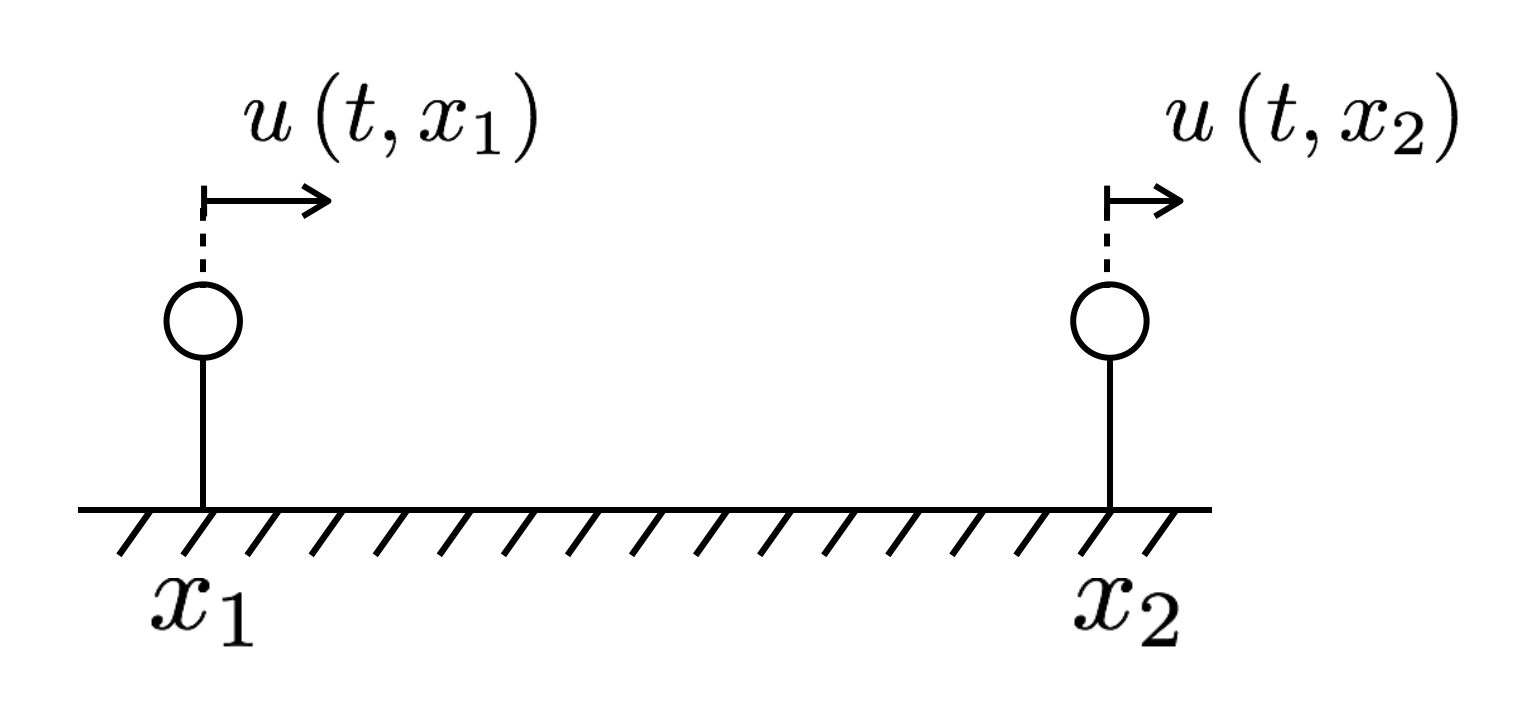
\includegraphics[width=11.0cm]{./img_cdmr_xarm.png}    
      \subcaption{3000 m distance in the X-arm}
      \label{img:img_cdmr_xarm}
    \end{minipage}
  \end{center}
  \begin{center}  
    \begin{minipage}{0.5\vsize}
      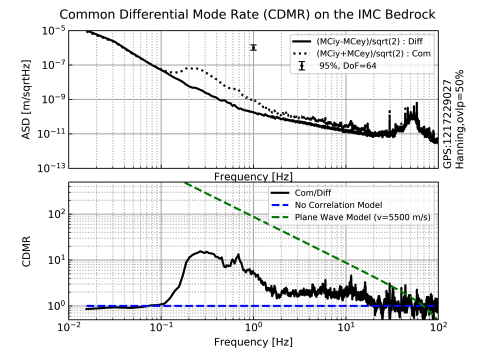
\includegraphics[width=11.0cm]{./img_cdmr_imc.png}
      \subcaption{30 m distance in the corner station}
      \label{img:img_cdmr_imc}  
    \end{minipage}
  \end{center}      
  \caption{\textbf{(Caution!! This plot shows the case of single plane wave.)} CDMRs in different distancies. (a) is measured in the X-arm. (b) is measured in the corner station. (Upper of each graph) The amplitude spectrum densities of the differential and the common motion which are measured by seismometers array drawn in Fig.(\ref{img:img_seismometer_map}). (Lower of each graph) The measured CDMR is shown in black line. Green Line is CDMR in the case the uniform plane wave model. Blue line is CDMR with no correlation between each the two points.}
\end{figure}


\begin{figure}[H]
  \begin{center}
    
\includegraphics[width=8cm]{./img_no_image.png}
  \end{center}
  \caption{}
  \label{img:img_seismometer_map}
\end{figure}






\subsection{Comparizon with Surface Detectors}
When length of the arm is almost the same, CDMR depends only on the phase velocity on of the ground, according to models in Eq.(\ref{eq:eq18}), Eq.(\ref{eq:eq20}). The phase Velocity is ...



\subsubsection{Phase Velocity Estimation}
I'm tired. I'll write tomorrow.
\begin{figure}[H] 
 \begin{minipage}{0.5\hsize}
  \begin{center}
    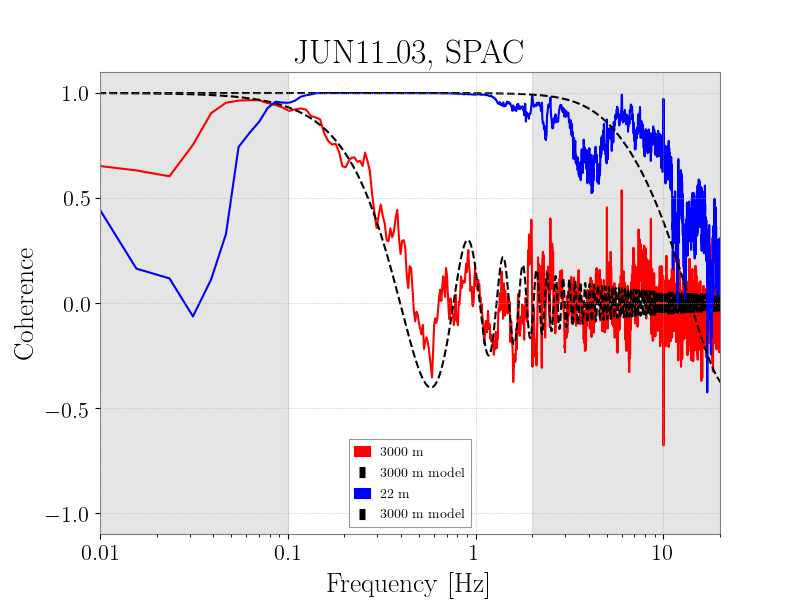
\includegraphics[width=8.0cm]{./img_coherence_result.png}    
  \end{center}
  \subcaption{}  
  \label{img:img_coherence_result}
 \end{minipage}
 \begin{minipage}{0.5\hsize}
  \begin{center}
    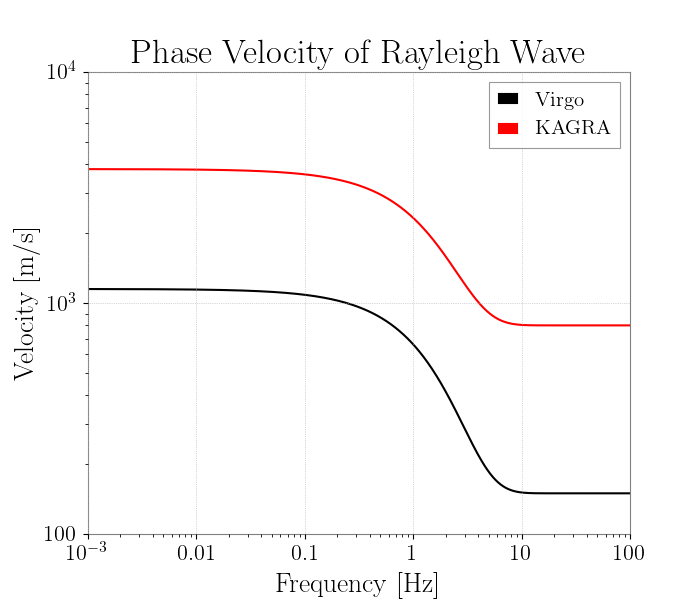
\includegraphics[width=8.0cm]{./img_RwaveVelocity.png}    
  \end{center}
  \subcaption{}
  \label{img:img_RwaveVelocity}  
 \end{minipage}
  \caption{(a) The complex coherence between two points. Red solid line is a complex coherence in 3000 m distance. Blue one is a coherence in 22 m distance. Black dashed line is given by Eq.(\ref{eq:eq19}) with asuming a profile of the phase velocity on Fig.(\ref{img:img_RwaveVelocity}). (b) The phase velocity of the Rayleigh wave. Black solid line is sited from M.Beker's PhD thesis. Red one is taken by fitting the measured data on Fig.(\ref{img:img_coherence_result})} 
\end{figure}

\subsubsection{}


\begin{figure}[H]
  \begin{center}
    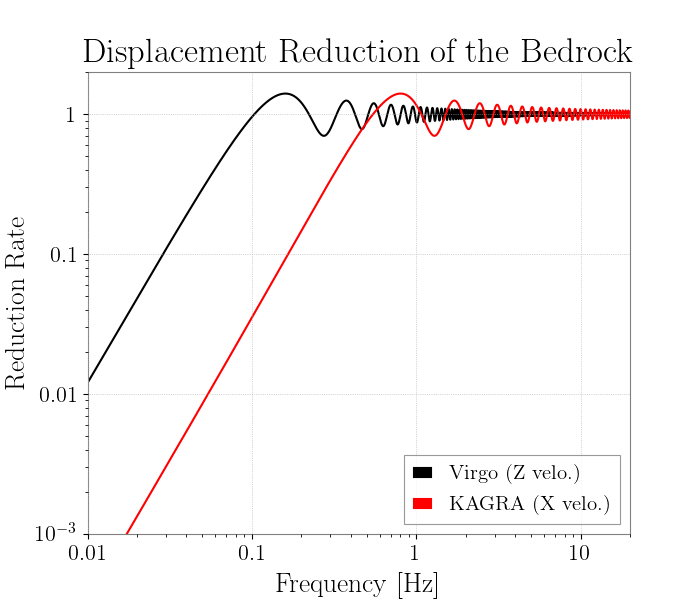
\includegraphics[width=9.5cm]{./img_CDMR.png}
  \end{center}
  \caption{Comparizon of the Reduction effect between KAGRA and Virgo. Differential motion represented in Eq.(\ref{eq:eq34}).   the phase velocity on the Fig.(\ref{img:img_RwaveVelocity})}
  \label{img:img_dmrr}
\end{figure}


\section{Summary of the Chapter}

\appendix

\bibliography{./cdmr_reference}

\end{document}
